\documentclass{beamer}
\usepackage[utf8]{inputenc}
\graphicspath{{./fig/}}

\title{Desenvolvimento Web Básico}
\subtitle{Aula 2}
\date{}

\usetheme{lucid}

\begin{document}
\frame{
 \titlepage
}

\frame{
    \frametitle{Roteiro de Aula}
    \tableofcontents
}


%---------------------------------------------------
\section{Listas}
\begin{frame}{Tags HTML - Listas}
  Listas são utilizada em diversas ocasiões em uma página HTML;
  \begin{itemize}
   \item A apresentação de itens do um assunto (como esse slide);
   \item Estruturação de novos componentes (como um menu);
  \end{itemize}
   Existem três tipos de listas no HTML:
  \begin{enumerate}
   \item Listas ordenadas;
    \item Listas não ordenadas;
    \item Listas de definições;
 \end{enumerate}
 Também é possível criar listas aninhadas.\\
 \tiny{Fonte: \cite{miletto2014desenvolvimento}}
\end{frame}
%---------------------------------------------------------------------------------
\subsection{Lista ordenada}
\begin{frame}{Lista ordenada}
  \begin{columns}
    \begin{column}{0.45 \textwidth}
     \begin{itemize}
      \item Cria uma lista que segue uma sequência numérica;
       \item Utiliza a tag $<$ol$>$ (\textit{ordered list});
       \item Cada item da lista é expresso entre a tag $<$li$>$ 
      (\textit{list item});
     \end{itemize}
    \end{column}
    \begin{column}{0.5\textwidth}
     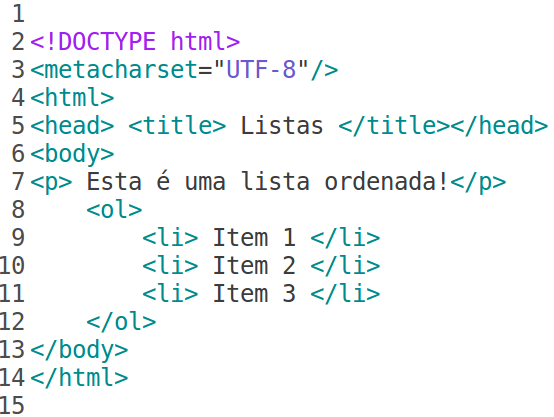
\includegraphics[height=0.45\paperheight]{fig/aula1/html2.png}
    \end{column}
  \end{columns}
\end{frame}
%---------------------------------------------------
\subsection{Lista desordenada}
\begin{frame}{Lista desordenada}
  \begin{columns}
    \begin{column}{0.45 \textwidth}
     \begin{itemize}
      \item Cria uma lista que não segue uma sequência.
       \item Utiliza a tag $<$ul$>$ (\textit{unordered list});
       \item Cada item da lista é expresso entre a tag $<$li$>$ 
      (\textit{list item});
     \end{itemize}
    \end{column}
    \begin{column}{0.5\textwidth}
     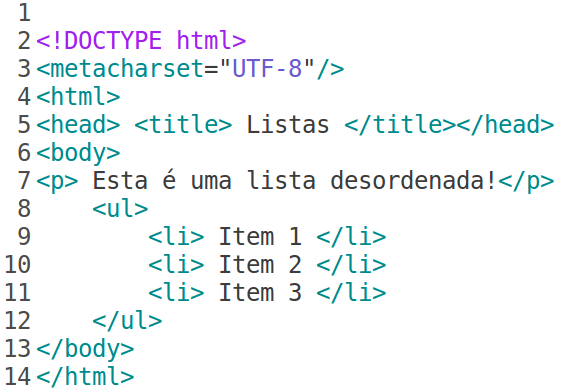
\includegraphics[height=0.45\paperheight]{fig/aula1/html3.png}
    \end{column}
  \end{columns}
\end{frame}
%----------------------------------------------------
\subsection{Lista de definição}
\begin{frame}{Lista de definição}
  \begin{columns}
    \begin{column}{0.45 \textwidth}
     \begin{itemize}
      \item Cria uma lista que define algum termo.
       \item Utiliza a tag $<$dl$>$ (\textit{definition list});
       \item Um termo é representado pela tag $<$dt$>$ 
(\textit{definition term});
       \item A definição é representada pela tag $<$dd$>$ 
      (\textit{definition definition});
       \item Uma $<$dt$>$ pode ter uma ou mais $<$dd$>$;
     \end{itemize}
    \end{column}
    \begin{column}{0.5\textwidth}
     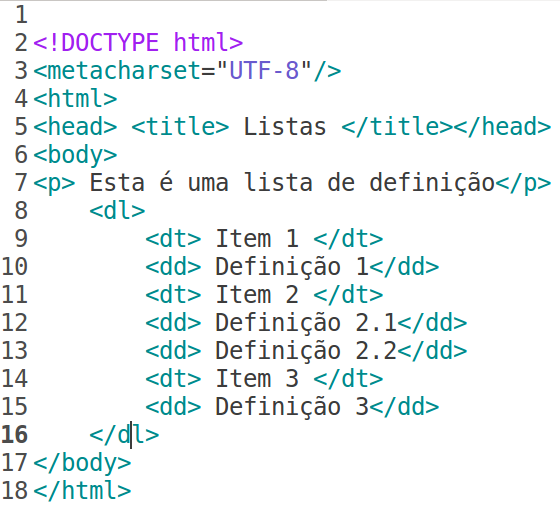
\includegraphics[height=0.55\paperheight]{fig/aula1/html4.png}
    \end{column}
  \end{columns}
\end{frame}
%-------------------------------------------------------------
\subsection{Listas aninhadas}
\begin{frame}{Listas aninhadas}
  \begin{columns}
    \begin{column}{0.45 \textwidth}
     \begin{itemize}
      \item Um item de uma lista pode se tornar uma nova lista;
       \item Essa estrutura representa uma sub lista de uma lista 
principal;
     \end{itemize}
    \end{column}
    \begin{column}{0.5\textwidth}
     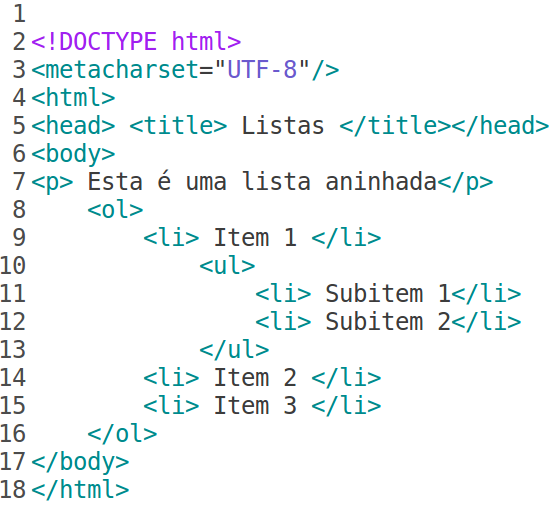
\includegraphics[height=0.55\paperheight]{fig/aula1/html5.png}
    \end{column}
  \end{columns}
\end{frame}
%-------------------------------------------------------------
\section{Âncoras (Links)}
\begin{frame}{Links}
  
  \begin{columns}
    \begin{column}{0.45 \textwidth}
  
      \begin{itemize}
      \item Permitem a movimentação entre páginas;
       \item Utilizado com a tag $<$a$>$;
       \item \textbf{href:} endereço da página na qual o link 
aponta; 
       \item mailto: abre a interface para envio de e-mail;
       \item \#id: uma parte específica da página;
       \item Download: link é um download;
     \end{itemize}
    \end{column}
    \begin{column}{0.5\textwidth}
     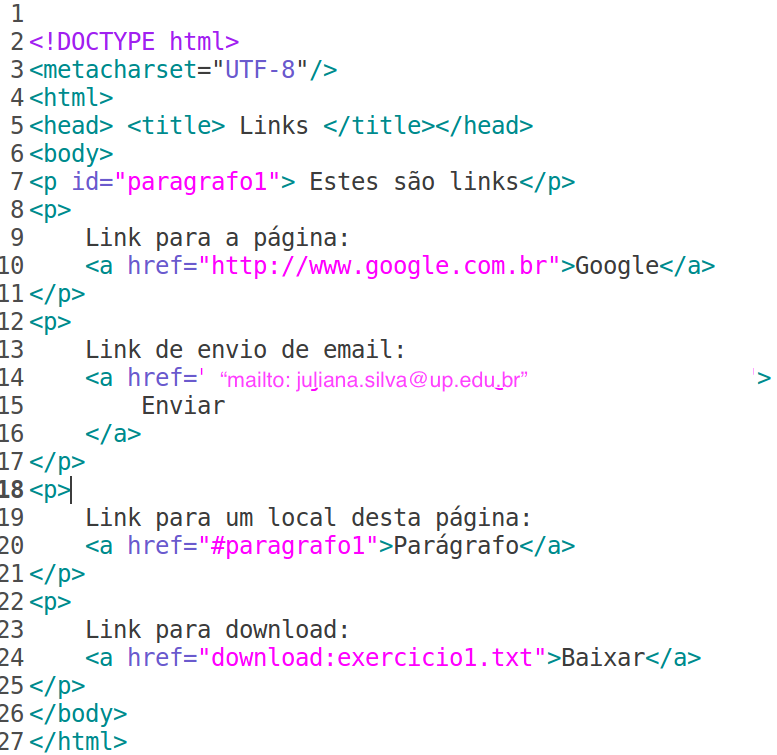
\includegraphics[height=0.6\paperheight]{fig/aula1/html6.png}
    \end{column}
  \end{columns}
\end{frame}
%--------------------------------------------------------------------------
\begin{frame}{Links}
  Parâmetros de link:
     \begin{itemize}
      \item \textbf{target:} especifica onde abrir o novo documento
       \item \_blank: abre em uma nova janela;
       \item \_self: abre onde o documento atual está (default); 
     \end{itemize}
     
     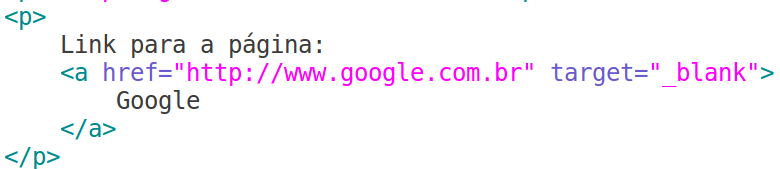
\includegraphics[height=0.25\paperheight]{fig/aula1/html7.png}
\end{frame}
%---------------------------------------------------------------------------
\section{Imagens}
\begin{frame}{Imagens}
  Adicionando imagens na página
  \begin{columns}
    \begin{column}{0.45 \textwidth}
     \begin{itemize}
      \item Representada pela tag $<$img$>$
       \item Parâmetros
      \begin{itemize}
	 \item \textbf{src:} aponta o caminho da imagem;
	 \item \textbf{alt:} indica um texto que substitui a imagem;
	 \item \textbf{title:} apresenta informação adicional sobre a 
imagem (tootip);
      \end{itemize}
    
     \end{itemize}
    
    \end{column}
    \begin{column}{0.5\textwidth}
     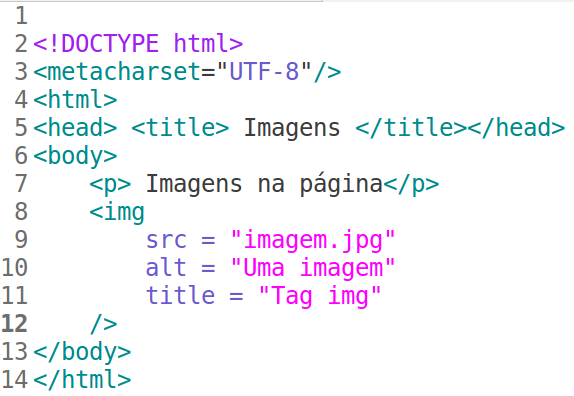
\includegraphics[height=0.45\paperheight]{fig/aula1/html8.png}
    \end{column}
  \end{columns}
\end{frame}
%---------------------------------------------------------------------------
\begin{frame}{Imagens}
  Adicionando imagens como links na página

     \begin{itemize}
      \item Você pode utilizar uma imagem como link
       \item Basta adicionar a tag $<$img$>$ dentro da tag $<$a$>$
     \end{itemize}
   

     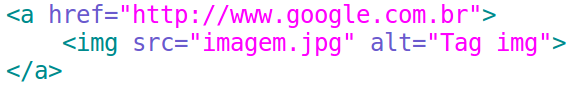
\includegraphics[height=0.15\paperheight]{fig/aula1/html9.png}
\end{frame}

%----------------AULA 3 Des. App-----------------------------------------------------------
\section{Marcações}
\begin{frame}{Atributo id}
  \begin{columns}
    \begin{column}{0.45 \textwidth}
      \small
     \begin{itemize}
      \item O atributo id serve para identificar unicamente um
elemento de uma página;
       \item Atributo global: qualquer tag do HTML pode possuir um id;
       \item Seu valor deve começar um uma letra ou um underline;
       \item Dois elementos em uma mesma página não podem possuir o mesmo 
id;
       \item Auxilia o CSS e o JavaScript;
     \end{itemize}
    \end{column}
    
    \begin{column}{0.5\textwidth}
     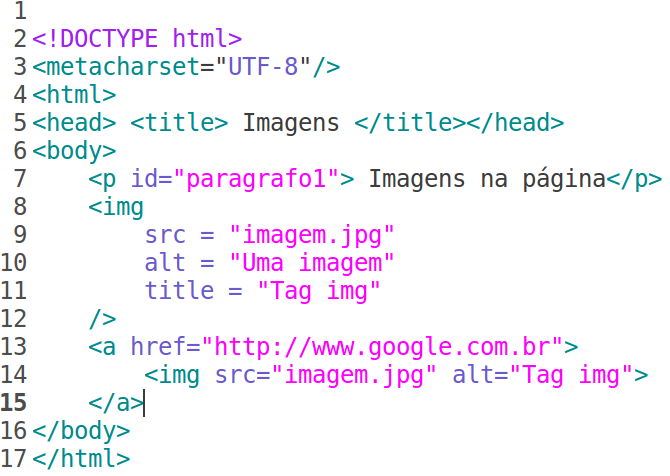
\includegraphics[height=0.45\paperheight]{fig/aula1/html10.png}
    \end{column}
  \end{columns}
\end{frame}
%---------------------------------------------------------------------------
\begin{frame}{Atributo class}
  \begin{columns}
    \begin{column}{0.45 \textwidth}
      \small
     \begin{itemize}
      \item O atributo class serve para categorizar um grupo de elementos com o 
mesmo comportamento;
       \item Atributo global: qualquer tag do HTML pode possuir um class;
       \item Seu valor deve começar um uma letra ou um underline;
       \item Auxilia o CSS e o JavaScript;
     \end{itemize}
    \end{column}
    
    \begin{column}{0.5\textwidth}
     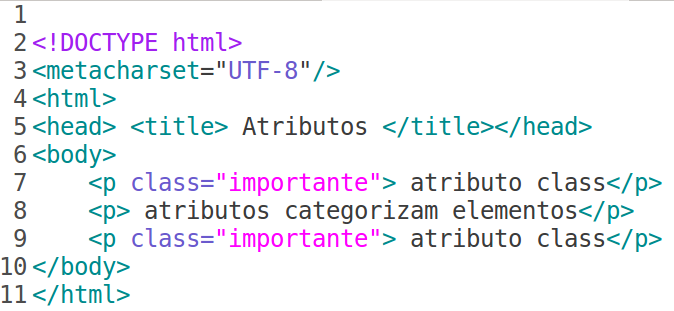
\includegraphics[height=0.3\paperheight]{fig/aula1/html11.png}
    \end{column}
  \end{columns}
\end{frame}
%---------------------------------------------------------------------------
\begin{frame}{Elementos: Block}
  Elementos Block
     \begin{itemize}
      \item Elementos que “sempre” são renderizados no começo de
uma nova linha;
     \end{itemize}
 
 Elementos Block em HTML
  \vspace{0.3cm}
 \begin{center}
     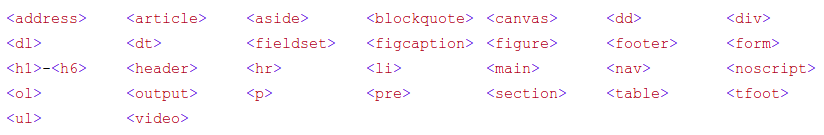
\includegraphics[height=0.18\paperheight]{fig/aula1/html12.png}
   \end{center}

\end{frame}
%---------------------------------------------------------------------------
\begin{frame}{Elementos: Inline}
  Elementos Inline
     \begin{itemize}
      \item Elementos que “sempre” são renderizados na mesma linha,
ao término de um elemento anterior;
     \end{itemize}
 
 Elementos InLine em HTML
 \vspace{0.3cm}
 \begin{center}
     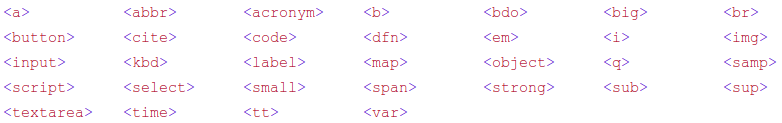
\includegraphics[height=0.18\paperheight]{fig/aula1/html13.png}
   \end{center}
\end{frame}
%---------------------------------------------------------------------------
\begin{frame}{Div}
  \begin{columns}
    \begin{column}{0.45 \textwidth}
      \small
     \begin{itemize}
       \item Permite o agrupamento de um conjunto de elementos em uma
box block-level;
       \item Cada conteúdo de uma div será apresentado em uma nova
linha;
       \item Esse comportamento pode ser alterado com CSS;
       \item Melhora a organização do código;
       \item É permitido colocar qualquer elemento dentro de uma div;
     \end{itemize}
    \end{column}
    
    \begin{column}{0.5\textwidth}
     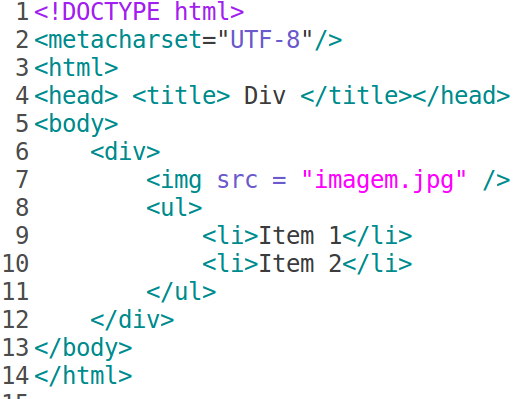
\includegraphics[height=0.5\paperheight]{fig/aula1/html14.png}
    \end{column}
  \end{columns}
\end{frame}
%--------------------------------------------------------------------
\section{Agrupando elementos}
\begin{frame}{Tag - Header}
  \begin{columns}
    \begin{column}{0.4 \textwidth}
      \small
      \begin{itemize}
	\item Utilizado para representar o cabeçalho de um documento ou seção;
	 \item Exemplo: cabeçalho de uma página;
      \end{itemize}
    \end{column}
    \begin{column}{0.55\textwidth}
     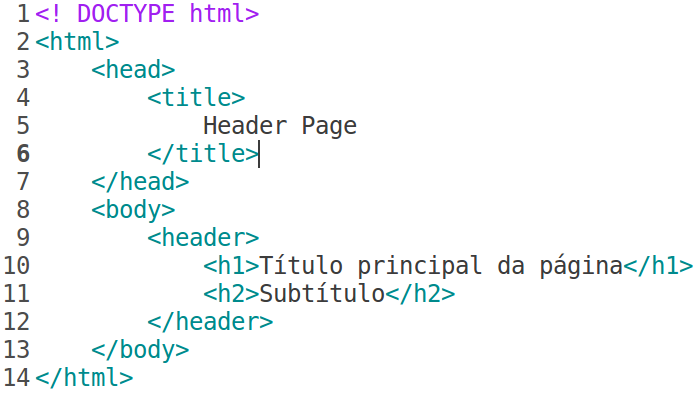
\includegraphics[height=0.4\paperheight]{fig/aula1/html15.png}
    \end{column}
  \end{columns}
\end{frame}
%-------------------------------------------------------------------------------
\begin{frame}{Tag - Section}
  \begin{columns}
    \begin{column}{0.4 \textwidth}
      \footnotesize
      \begin{itemize}
	\item Representa uma seção dentro de um documento.
	 \item Utiliza-se essa tag para descrever separadamente as seções 
e tópicos de um documento;
	 \item O conjunto de seções completam a relevância do conteúdo do 
documento, como seções de um artigo de um blog;
      \end{itemize}
    \end{column}
    \begin{column}{0.6\textwidth}
     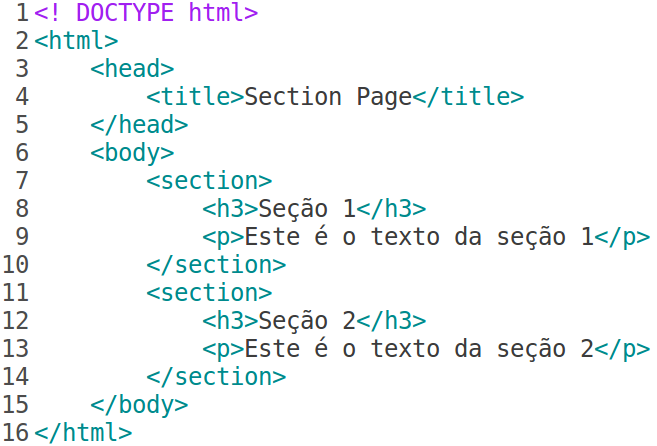
\includegraphics[height=0.4\paperheight]{fig/aula1/html16.png}
    \end{column}
  \end{columns}
  \textcolor{red}{Salve esse código em um arquivo chamado 1.html}
\end{frame}
%-------------------------------------------------------------------------------
\begin{frame}{Tag - Main}
  \begin{columns}
    \begin{column}{0.4 \textwidth}
      \footnotesize
      \begin{itemize}
	\item Utilizado para especificar o conteúdo principal, de maior
relevância, de um documento;
	 \item Cada página deve apresentar apenas um conteúdo principal;
	 \item Exemplo: espaço reservado para a apresentação do conteúdo 
de um blog;
      \end{itemize}
    \end{column}
    \begin{column}{0.6\textwidth}
     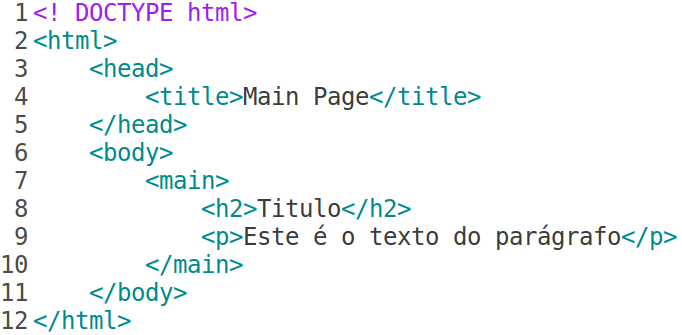
\includegraphics[height=0.35\paperheight]{fig/aula1/html19.png}
    \end{column}
  \end{columns}
  \textcolor{red}{Salve esse código em um arquivo chamado 2.html}
\end{frame}
%-------------------------------------------------------------------------------
\begin{frame}{Tag - Aside}
  \begin{columns}
    \begin{column}{0.4 \textwidth}
      \footnotesize
      \begin{itemize}
	\item Utilizado para criar um conteúdo de apoio, ou adicional,
ao conteúdo principal;
	 \item Exemplo: artigos com temas relacionados de um blog;
      \end{itemize}
    \end{column}
    \begin{column}{0.6\textwidth}
     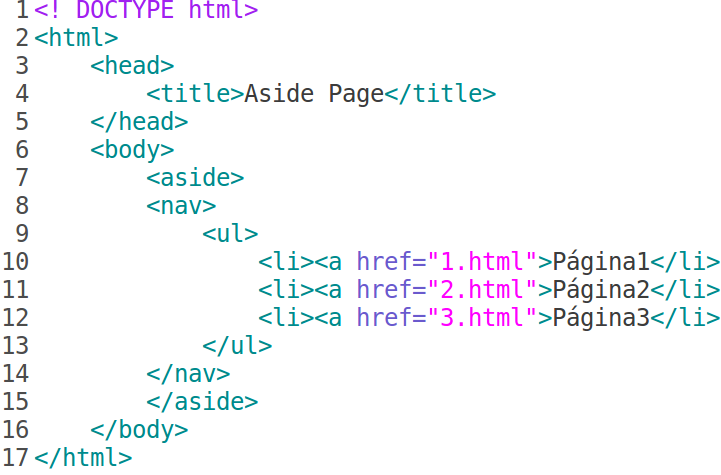
\includegraphics[height=0.45\paperheight]{fig/aula1/html18.png}
    \end{column}
  \end{columns}
  \textcolor{red}{Salve esse código em um arquivo chamado 3.html}
\end{frame}
%-------------------------------------------------------------------------------
\begin{frame}{Tag - Nav}
  \begin{columns}
    \begin{column}{0.35 \textwidth}
      \footnotesize
      \begin{itemize}
	\item Utilizado para representar um agrupamento de links de
navegação;
	 \item Exemplo: paginação de uma busca;
      \end{itemize}
    \end{column}
    \begin{column}{0.65\textwidth}
     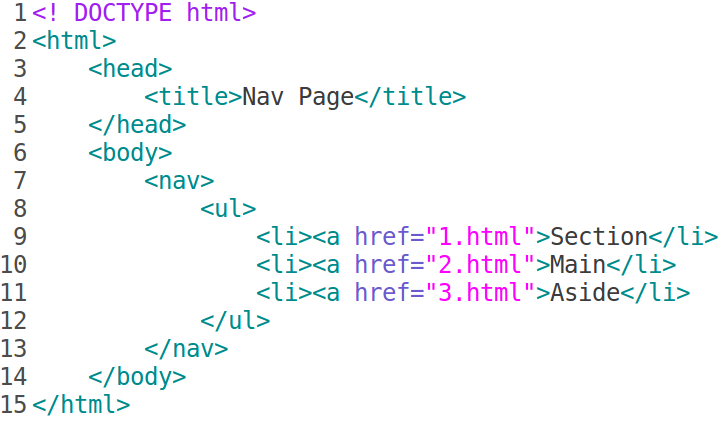
\includegraphics[height=0.43\paperheight]{fig/aula1/html17.png}
    \end{column}
  \end{columns}
\end{frame}
%----------------------------------------------------
\section{Atividade de aula}
\begin{frame}{Atividade de aula}
\begin{block}{Atividade de aula 2}
    \begin{enumerate}
        \item Desenvolva uma página HTML (index.html) que explique os fundamentos do HTML (conteúdo da aula 1 e 2);
        \item Na página index.html crie dois links para outras duas páginas (page1.html e page2.html), um link deve ser em forma texto, o outro link deve ser uma imagem;
        \item Crie 3 seções na página index.html, uma sobre Tags, uma sobre listas, outra sobre imagens e links;
        \item Desenvolva um menu na página index.html o menu deve encaminhar o usuário para as seções criadas no item anterior;
    \end{enumerate}
\end{block}
    
\end{frame}
%-----------------------------------------------------
\section{Leitura recomendada}
\begin{frame}{Leitura complementar [1]}
 Para mais informações sobre HTML e CSS, leia:\\
 \begin{columns}
   \begin{column}{0.5\textwidth}
    Desenvolvimento de Software II: Introdução ao Desenvolvimento Web com HTML, CSS, JavaScript e PHP \\
     Capítulo 4 - Página 61\\ 
      \cite{miletto2014desenvolvimento}
   \end{column}
   \begin{column}{0.3\textwidth}
    \begin{center}
  
\includegraphics[height=0.45\paperheight]{fig/aula2/milleto2014.jpeg} \\
 \end{center}
   \end{column}
 \end{columns}
\end{frame}

%-----------------------------------------------------
\begin{frame}{Leitura complementar [2]}
 Para mais informações sobre HTML5, leia:\\
 \begin{columns}
   \begin{column}{0.4\textwidth}
     HTML5 - Embarque imediato\\ 
      \cite{flatschart2011html}
   \end{column}
   \begin{column}{0.3\textwidth}
    \begin{center}
  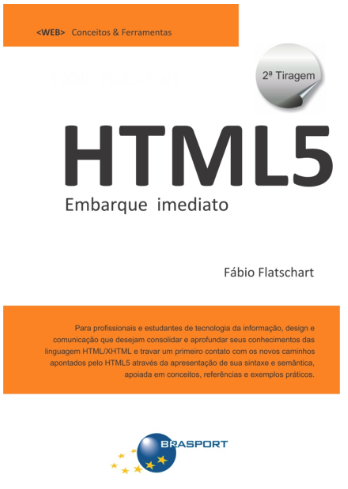
\includegraphics[height=0.5\paperheight]{fig/aula2/flatschart2014html.png} \\
 \end{center}
   \end{column}
 \end{columns}
\end{frame}
%---------------------------------------------------------------------
\section{Referências}
\begin{frame}{Referências}%[allowframebreaks]
\frametitle{Referências}
\small
\begin{center}
\tiny
\bibliographystyle{apalike}
\bibliography{./ref_aula}
\end{center}
\end{frame}


\end{document}